\chapter{\label{ref:PARTII}The Rockbox interface}
\section{Your Jukebox}
\begin{figure}[h!]
\begin{center}
\opt{player}{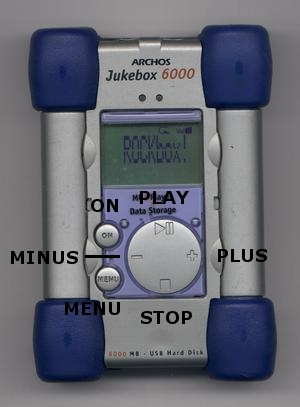
\includegraphics[height=11.8cm]{rockbox_interface/images/player-front.png}}
\opt{recorder,recorderv2fm}{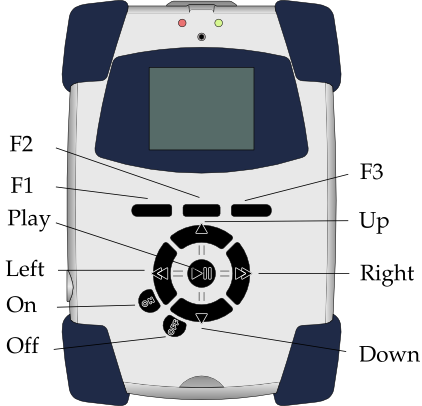
\includegraphics[height=11.8cm]{rockbox_interface/images/recorderv2fm-front.png}}
\opt{ondio}{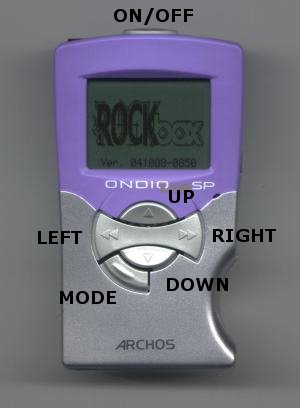
\includegraphics[height=11.8cm]{rockbox_interface/images/ondio-front.png}}
\opt{h1xx}{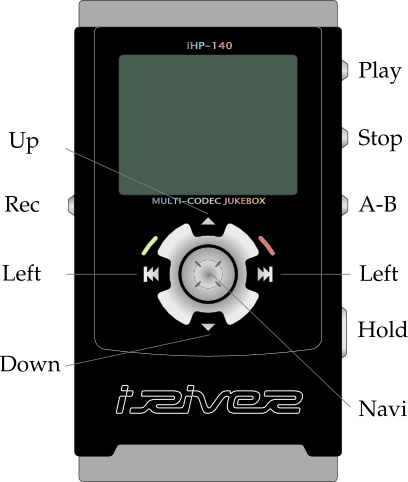
\includegraphics[height=11.8cm]{rockbox_interface/images/h1xx-front.png}}
\end{center}
\caption{\playerman \vspace{1cm} \playertype}
\end{figure}

Throughout this manual, the buttons on the Jukebox are labelled
according to the pictures above.  There are minor cosmetic differences
between Jukebox models, but the buttons are in approximately the same
position as on the picture.\\

To turn on a Jukebox containing Rockbox, hold down the ON key
for 2{}-3 seconds.  (Flashed Jukeboxes only require a tap of the ON key
{--} see page \textup{\pageref{ref:FlashingRockboxReal}} for more
information about flashing Rockbox.) 
\label{ref:Safeshutdown}On shutdown, Rockbox automatically saves its settings and turns off the hard drive safely. To tell Rockbox to shut the Jukebox down, do the following:


\begin{table}[h!]
  \begin{center}
    \begin{tabular}{@{}lc@{}}\toprule
      \textbf{Model} & \textbf{Power Off} \\\midrule
      V2 / FM RECORDER/ ONDIO & Hold  the OFF key for 2{}-3 seconds \\
      V1 RECORDER & Double{}-tap the OFF key when playback is stopped \\
      PLAYER & From the Rockbox Main Menu select \textbf{Shutdown} \\\bottomrule
    \end{tabular}
  \end{center}
\end{table}

In the unlikely event of a software failure, a hardware power off can be
performed by holding down STOP until the Jukebox power light goes off. 
This works for all models of Jukebox.\\

For further details about connecting, charging and caring for your
Jukebox, please see the Archos manual that came with it.

\section{\label{ref:PartIIFB}File Browser}
{\centering\itshape
  [Warning: Image ignored] % Unhandled or unsupported graphics:
%\includegraphics[width=4.15cm,height=2.35cm]{images/rockbox-manual-img11.png}
     [Warning: Image ignored] % Unhandled or unsupported graphics:
%\includegraphics[width=4.15cm,height=1.981cm]{images/rockbox-manual-img12.png}
 \newline
Recorder file browser  Player file browser  
\par}
The file browser helps you navigate through the files on your Jukebox,
entering folders and executing the default action on each file. To help
us differentiate files, each file format is displayed with an icon. You
can select which file types are displayed (see page
\pageref{ref:ShowFiles}).

\subsection{\label{ref:PartIISectionCtrls}Controls}
\opt{Rec}{
  \begin{table}[h!]
    \begin{center}
      \begin{tabular}{@{}cc@{}}\toprule
        \textbf{Key} & \textbf{Function} \\\midrule
        %
        UP/DOWN & Go to previous/next item in list. \\
                & If you are on the first/last entry, \\
                & the cursor will wrap to the last/first entry. \\
        %
        ON+UP/DOWN & Move one page up/down on the list.\\
        %
        LEFT & Go to the parent directory. \\
        %
        PLAY/RIGHT & Executes an action. \\
                   & Depending on the file type, that action may vary. \\
                   & (See page \pageref{ref:Filemenu}) \\
        %
        Centering & If there is a MP3 playing, \\
                  & returns to the While Playing Screen (WPS) \\
                  & without stopping playback.  \\
        %
        ON+PLAY/HOLD PLAY & Enters the File Menu \\
        %
        F1 & Switches to the Main Menu \\
        %
        F2 & Switches to the Browse/Play Quick Menu \\
        %
        F3 & Switches to the Display Quick Menu \\ \bottomrule
        %
      \end{tabular}
    \end{center}
  \end{table}
}
%
\opt{PS}{
  \begin{table}[h!]
    \begin{center}
      \begin{tabular}{@{}cc@{}}\toprule
        \textbf{Key} & \textbf{Function} \\\midrule
        MINUS/PLUS & Go to previous/next item in list. \\
                   & If you are on the first/last entry, \\
                   & the cursor will wrap to the last/first entry. \\
        STOP & Go to the parent directory. \\
        PLAY & Executes an action. \\
             & Depending on the file type, that action may vary.\\
             & (See page \pageref{ref:Filemenu}) \\
        ON & If there is a MP3 playing, \\
           & returns to the While Playing Screen (WPS) \\
           & without stopping playback. \\
        ON+PLAY/HOLD PLAY & Enters the File Menu \\
        Menu & Switches to the Main Menu \\\bottomrule
      \end{tabular}
    \end{center}
  \end{table}
  The functions of the F keys are also summarised on the button bar at the
  bottom of the screen.
}


\subsection{\label{ref:Filemenu}\label{ref:PartIISectionFM}File Menu}
{\centering\itshape
  [Warning: Image ignored] % Unhandled or unsupported graphics:
%\includegraphics[width=4.15cm,height=2.35cm]{images/rockbox-manual-img13.png}
     [Warning: Image ignored] % Unhandled or unsupported graphics:
%\includegraphics[width=4.15cm,height=1.951cm]{images/rockbox-manual-img14.png}
 \newline
Recorder file menu  Player file menu  
\par}

This menu operates on the file that was selected in the browser at the
time ON+PLAY was pressed to enter it.  It can also be accessed by
holding down the PLAY key for a short while.  It offers the following
options:

\begin{itemize}
\item \textbf{Open with:} Runs a viewer plugin on the file. 
Normally the filetype of a file is detected and the appropriate plugin
is run automatically when you press play on it.  Use this menu if for
some reason you want to override the default action and select a viewer
by hand.  See page \textmd{\pageref{ref:Viewersplugins}} for more details on viewers.
For example, this would be used to run the VBRfix plugin to recreate the
Xing header for an MP3 file, which can fix problems such as
fast{}-forward and rewind not working correctly on a particular MP3 file or the play time of a track being listed incorrectly. 
\item \textbf{Playlist:} Change to the Playlist submenu (see below).
\item \textbf{Rename:} This function lets the user modify a file name.
\item \textbf{Delete:} Only files can be deleted, not folders. Rockbox will ask for confirmation before deleting a file. Press PLAY to confirm deletion or any other key to cancel.
\item \textbf{Delete Directory: }Deletes the folder pointed to by the cursor and all the files and folders contained in it.  Use with caution.
\item \textbf{Create Directory:} Makes a new folder in the current folder on
the disk.
\end{itemize}


\subsection{\label{ref:Playlistsubmenu}Playlist Submenu}
If the playlist submenu is invoked on a directory, it will act on all the files within that directory.  If invoked on a playlist it will act on all the files in that playlist. Otherwise it acts only on the current file.

{\centering\itshape
  [Warning: Image ignored] % Unhandled or unsupported graphics:
%\includegraphics[width=4.15cm,height=2.35cm]{images/rockbox-manual-img15.png}
     [Warning: Image ignored] % Unhandled or unsupported graphics:
%\includegraphics[width=4.15cm,height=1.951cm]{images/rockbox-manual-img16.png}
 \newline
  Recorder playlist submenu  Player playlist submenu
\par}

This menu provides the following options:

\begin{itemize}
\item \textbf{Insert:} Add track(s) to playlist. If no other tracks have been
inserted then the selected track will be added immediately after
current playing track, otherwise they will be added to end of insertion
list.
\item \textbf{Insert next: }Add track(s) immediately after current playing
track, no matter what else has been inserted.
\item \textbf{Insert last: }Add track(s) to end of playlist.
\item \textbf{Queue: } Queue is the same as Insert except queued
tracks are deleted immediately from the playlist after
they've been played. Also, queued tracks are not saved to the playlist file (see page \pageref{ref:playlistoptions}).
\item \textbf{Queue next:} Queue track(s) immediately after current playing
track.
\item \textbf{Queue last: }Queue track(s) at end of playlist.
\end{itemize}

You can insert a track, directory or playlist even if nothing is
currently playing. In this case, a new playlist is created with only
the selected tracks and then play is started.

Note: The dynamic playlist is saved so resume will restore it exactly as
before shutdown. Stopped playlists can be resumed from File Browser by
pressing ON.




\subsection{Virtual Keyboard}
{\centering\itshape
  [Warning: Image ignored] % Unhandled or unsupported graphics:
%\includegraphics[width=4.165cm,height=2.177cm]{images/rockbox-manual-img17.png}
 \textmd{  }  [Warning: Image ignored]
% Unhandled or unsupported graphics:
%\includegraphics[width=4.598cm,height=2.071cm]{images/rockbox-manual-img18.png}
 \newline
  Recorder keyboard  Player Keyboard  
\par}

This is the virtual keyboard that is used when entering file names in
Rockbox.

\opt{Rec}{
  \begin{table}[h!]
    \begin{center}
      \begin{tabular}{@{}cc@{}}\toprule
        \textbf{Key} & \textbf{Function} \\\midrule
        ARROW KEYS & Move about the virtual keyboard \\
                   & (moves the solid cursor) \\
        ON+LEFT/RIGHT & Move about within the current file name \\
                      & (moves the line cursor) \\
        PLAY & Inserts the currently selected keyboard letter \\
             & at the current filename cursor position \\
        STOP & Exits the virtual keyboard without saving any changes \\
        ON & No action \\
        F1 & SHIFT: Shifts between the upper case, \\
           & lower case and accented keyboards \\
        F2 & OK: Exits the virtual keyboard and saves any changer \\
        F3 & DEL: Deletes the character before\\ 
           & the current filename cursor \\\bottomrule
      \end{tabular}
    \end{center}
  \end{table}
}


\opt{PS}{
  The current filename is always listed on the first line of the display. 
  The second line of the display can contain the character selection bar,
  as in the screenshot above, or  one of a number of other options.
  
  \begin{table}[h!]
    \begin{center}
      \begin{tabular}{@{}cc@{}}\toprule
        \textbf{Key} & \textbf{Function} \\\midrule
        MINUS/PLUS & Moves the arrow to/from the filename \\
                   & and changes between the character bar \\
                   & and BACKSPACE, DELETE, ACCEPT and ABORT. \\
        PLAY/STOP & Varies (see below) \\
        ON & Nothing \\
        Menu & Shift.  When the character selection bar is selected\\
             & this changes between upper case, lower case, \\
             & and accented letters. \\\bottomrule
      \end{tabular}
    \end{center}
  \end{table}
  The function of the PLAY and STOP buttons depends on what the arrow is
  pointing to, as follows.
  
  \begin{table}[h!]
    \begin{center}
      \begin{tabular}{@{}cc@{}}\toprule
        \textbf{Selected option} & \textbf{Play/Stop function} \\\midrule
        filename & Moves the cursor left (STOP) \\
                 & or right (PLAY) within the filename \\
        character bar & Moves the character bar to the next (PLAY)\\
                      & or previous (STOP) character. \\
        BACKSPACE & PLAY deletes the character before \\
                  & the current cursor position \\
        DELETE & PLAY deletes the character at the \\
               & current cursor position\\
        ACCEPT & PLAY exits the virtual keyboard and \\
               & saves any changes \\
        ABORT & PLAY exits the virtual keyboard and \\
              & discards any changes \\\bottomrule
      \end{tabular}
    \end{center}
  \end{table}
}

\section{\label{ref:WPS}\label{ref:PartIISectionWPS}While Playing
Screen}
The While Playing Screen (WPS) displays various pieces of information
about the currently playing MP3 file:
%
\opt{Rec}{
\begin{itemize}
\item Status bar: Battery level, charger status, volume, play mode, repeat
mode, shuffle mode and clock.
\item Scrolling path+filename of the current song.
\item The ID3 track name.
\item The ID3 album name.
\item The ID3 artist name.
\item Bit rate. VBR files display average bitrate and ``(avg)''
\item Elapsed and total time.
\item A slidebar progress meter representing where in the song you are.
\item Peak meter.
\end{itemize}

Notes:

\begin{itemize}
\item The number of lines shown depends on the size of the font used.
\item The peak meter is only visible if you turn off the status bar or if
using a small font that gives 8 or more display lines.
\end{itemize}
}
%
\opt{PS}{
\begin{itemize}
\item Playlist index/Playlist size: Artist {}- Title.
\item Current{}-time Progress{}-indicator Left.
\end{itemize}

See page \textmd{\pageref{ref:ConfiguringtheWPS}} for
details of customising your WPS (While Playing Screen).
}

\subsection{\label{ref:PartIISectionWPSCtrls}WPS Key Controls}

\opt{Rec}{
  \begin{table}[h!]
    \begin{flushleft}
      \begin{tabular}{@{}cc@{}}\toprule
        \textbf{Key} & \textbf{Action} \\\midrule
        UP/DOWN & Volume up/down \\
        LEFT & (quick press) Go to beginning of track, \\
             & or if pressed while in the first seconds of a track, \\
             & go to previous track \\
        LEFT (hold) & Rewind in track \\
        RIGHT & (quick press) Go to next track. \\
        RIGHT (hold) & Fast forward in track. \\
        PLAY & Toggle play/pause \\
        ON & (quick press) Go to file browser \\
        ON (hold) & Show pitch setting screen \\
        STOP & Stop playback \\
        F1 & Go to Main menu \\
        F2 & Toggles Play/browse quick menu \\
        F3 & Toggles Display quick menu \\
        F1+DOWN & Key lock on/off \\
        F1+PLAY & Mute on/off \\
        F1+ON & Enter ID3 viewer \\\bottomrule
      \end{tabular}
    \end{flushleft}
  \end{table}
}
%
\opt{PS}{
  \begin{table}[h!]
    \begin{center}
      \begin{tabular}{@{}cc@{}}\toprule
        \textbf{Key} & \textbf{Action} \\\midrule
        MENU+PLUS & Increases volume \\
        MENU+MINUS & Decreases volume \\
        MINUS & (quick press) Go to beginning of track, \\
              & or if pressed while in the first seconds of a track, \\
              & go to previous track. \\
        MINUS (hold) & Rewind in track \\
        PLUS & (quick press) Go to next track. \\
        PLUS (hold) & Fast{}-forward in track. \\
        PLAY & Toggle play/pause \\
        ON & Quick press = Go to file browser \\
        OFF & Stop playback \\
        MENU & Go to Main menu \\
        MENU+STOP & Key lock on/off \\
        MENU+PLAY & Mute on/off \\
        MENU+ON & Enter ID3 viewer \\\bottomrule
      \end{tabular}
    \end{center}
  \end{table}
}

\opt{Rec,Rec2,FMRec,OndioSP,OndioFM,H120}{
\subsection{Peak Meter}
The peak meter can be displayed on the While Playing Screen and consists
of several indicators.  For a picture of the peak meter, please see the
While Recording Screen on page \pageref{ref:Whilerecordingscreen}.

\begin{itemize}
\item \textbf{The bar: }This is the wide horizontal bar. It represents the
current volume value.
\item \textbf{The peak indicator:} This is a little vertical line at the right
end of the bar. It indicates the peak volume value that occurred
recently.
\item \textbf{The clip indicator: }This is a little black block that is
displayed at the very right of the scale when an overflow occurs. It
usually doesn't show up during normal playback unless
you play an audio file that is distorted heavily. If you encounter
clipping while recording your recording will sound distorted. You
should lower the gain. Note that the clip detection is not very
precise. Clipping might occur without being indicated.
\item \textbf{The scale: }Between the indicators of the right and left channel
there are little dots. These dots represent important volume values. In
linear mode each dot is a 10\% mark. In dbfs mode the dots represent
the following values (from right to left): 0db, {}-3db, {}-6db, {}-9db,
{}-12db, {}-18db, {}-24db, {}-30db, {}-40db, {}-50db, {}-60db.
\end{itemize}
}

\subsection{\label{ref:ID3viewer}ID3 Viewer}
{\centering\itshape
  [Warning: Image ignored] % Unhandled or unsupported graphics:
%\includegraphics[width=3.833cm,height=2.191cm]{images/rockbox-manual-img21.png}
 \newline
The ID3 viewer
\par}

This screen is accessible from the WPS screen by pressing F1+ON (recorder) or MENU+ON (player).  It provides a detailed view of all the identity information about the current track that is stored in an MP3 file.  Use the LEFT and RIGHT (recorder) or PLUS and MINUS (player) keys to move through the information and the STOP key to exit the viewer.


\opt{Rec,Rec2,FMRec,H120}{
\section{\label{ref:QuickScreenMenus}Quick Screen Menus}

{\centering\itshape
  [Warning: Image ignored] % Unhandled or unsupported graphics:
%\includegraphics[width=4.15cm,height=2.35cm]{images/rockbox-manual-img22.png}
 \textmd{  }  [Warning: Image ignored]
% Unhandled or unsupported graphics:
%\includegraphics[width=4.15cm,height=2.35cm]{images/rockbox-manual-img23.png}
 \newline
F2 Quick Screen Menu  F3 Quick Screen Menu
\par}

Rockbox handles function buttons in a different way to the Archos
software. F1 is always bound to the menu function, while F2 and F3
enable two quick menus.  

F2 displays some browse and play settings which are likely to be changed
frequently. This settings are Shuffle mode, Repeat mode and the Show
files options

Shuffle mode plays each track in the currently playing list in a random
order rather than in the order shown in the browser.

Repeat mode repeats either a single track (One) or the entire playlist
(All).

Show files determines what type files can be seen in the browser.  This
can be just MP3 files and directories (Music), Playlists, MP3 files and directories  (Playlists), any files that Rockbox supports (Supported) or all files on the disk (All).

See page \pageref{ref:PlaybackOptions} for more information about these
settings.

\begin{table}[h!]
  \begin{center}
    \begin{tabular}{@cc@{}}\toprule
      \textbf{Key} & \textbf{Action} \\\midrule
      LEFT & Controls Shuffle mode setting \\
      RIGHT & Controls Repeat mode setting \\
      DOWN & Controls Show file setting \\\bottomrule
    \end{tabular}
  \end{center}
\end{table}
F3 controls frequently used display options.

Scroll bar turns the display of the Scroll bar on the left of the screen
on or off.

Status bar turns the status display at the top of the screen on or off.

Upside down inverts the screen so that the top of the display appears
nearest to the buttons.  This is sometimes useful when storing the
Jukebox in a pocket.  Key assignments swap over with the display
orientation where it is logical for them to do so.

See page \pageref{ref:Displayoptions} for more information about these
settings.

\begin{table}[h!]
  \begin{center}
    \begin{tabular}{@{}cc@{}}\toprule
      \textbf{Key} & \textbf{Action} \\\midrule
      LEFT & Controls scroll bar display \\
      RIGHT & Controls status bar display \\
      DOWN & Controls upside down screen setting \\\bottomrule
    \end{tabular}
  \end{center}
\end{table}
}
